\documentclass[conference]{IEEEtran}
\usepackage{graphicx}
\usepackage{booktabs}
\usepackage{amsmath}
\usepackage{hyperref}
\usepackage{caption}
\usepackage{subcaption}
\usepackage{url}

\title{SceneIQ: Detecting Logical Inconsistencies in Photographs Using Vision Transformer and Scene-Graph Fusion}

\author{
\IEEEauthorblockN{Siddhi Rohan Chakka}
\IEEEauthorblockA{UID: 121302823\\University of Maryland}
\and
\IEEEauthorblockN{Krishna Kishore Buddi}
\IEEEauthorblockA{UID: 121142672\\University of Maryland}
\and
\IEEEauthorblockN{Dhanush Vasa}
\IEEEauthorblockA{UID: 121227645\\University of Maryland}
}

\begin{document}

\maketitle

% ============================================================================
\begin{abstract}
SceneIQ detects logically inconsistent elements in photographs by fusing visual features with scene-graph structure. Given a single RGB image, it classifies the scene as coherent or incoherent and produces a heatmap showing where the anomaly is. We built a benchmark of 15,000 images from Visual Genome: 10,000 real photographs and 5,000 synthetic composites where out-of-place objects are pasted into scenes based on co-occurrence statistics. The model pairs a Vision Transformer (ViT) backbone with a Graph Attention Network (GAT) encoder via cross-attention. On the test set, the fusion model reaches 94.4\% accuracy and 91.6\% F1, beating the ViT-only baseline (91.5\% F1). A GAT-only model collapses to majority-class prediction (66.7\% accuracy), confirming that visual features carry most of the signal. Adding a localization loss over ground-truth bounding boxes brings pointing accuracy to 86.9\% (up from 12.9\% without it). Code and trained weights are at \url{https://github.com/SiddhiRohan/sceneiq}.
\end{abstract}

% ============================================================================
\section{Introduction}

Object detection and segmentation have gotten very good, but most vision systems never ask whether a scene actually makes sense. A penguin sitting in a kitchen or a boat in a desert would not raise any flags for a standard detector. Humans spot these immediately. The question we are interested in is whether a model can too.

This matters for image forensics and for checking outputs of generative models, where semantic errors (objects in wrong contexts) are common but pixel-level artifacts may not be. Prior out-of-distribution detection work~\cite{johnson2015image,xu2017scene} tends to focus on pixel statistics or distribution shifts rather than the relationships between objects in a scene.

SceneIQ approaches this as a classification problem: given a single RGB photograph, decide whether the scene is coherent or incoherent, and if incoherent, point to where the problem is. We pair a Vision Transformer~\cite{dosovitskiy2020image} with a Graph Attention Network~\cite{velickovic2018graph} that encodes scene-graph relationships, and fuse them through cross-attention. We also construct a benchmark from Visual Genome~\cite{krishna2017visual} using co-occurrence-guided copy-paste to generate incoherent samples, and add a per-patch localization head trained against ground-truth bounding boxes.

% ============================================================================
\section{Methodology}

\subsection{Dataset Construction}

We build our benchmark from Visual Genome (VG), which provides 108,077 images with dense scene graph annotations including objects, attributes, and relationships.

\textbf{Co-occurrence mining.} We compute pairwise object co-occurrence counts across all VG scene graphs. Object pairs that appear together fewer than 10 times are considered rare. When an object that is rare for a given scene is pasted into it, the result is an incoherent composition.

\textbf{Synthetic incoherent images.} We generate 5,000 incoherent images using copy-paste augmentation. For each sample, we select a destination scene and an alien object category that rarely co-occurs with the scene's existing objects. We crop the alien object from a different VG image and paste it into the destination at a random location. Quality filters ensure: (a) the alien category has at least 50 VG instances, and (b) the crop is at least 32$\times$32 pixels. The acceptance rate is 48\% (5,000 accepted from 10,372 attempts). Each sample records the paste bounding box for localization evaluation.

\textbf{Dataset splits.} The final dataset has 10,000 coherent images (real VG photographs) and 5,000 incoherent images, split 70/15/15 into train (10,500), validation (2,250), and test (2,250) sets with stratified sampling. To prevent data leakage, VG images used as paste destinations are excluded from the coherent pool.

\subsection{Model Architecture}

Our fusion model has three components (Figure~\ref{fig:architecture}):

\textbf{ViT backbone.} We use \texttt{google/vit-base-patch16-224}, pretrained on ImageNet-21k~\cite{dosovitskiy2020image}. The image is divided into a 14$\times$14 grid of 16$\times$16 patches, producing 196 patch token embeddings of dimension 768.

\textbf{GAT encoder.} Scene graph nodes represent object categories, embedded via a learned embedding layer (dimension 128). Relationships form edges in the graph. We apply 2 layers of Graph Attention Convolution~\cite{velickovic2018graph} with 4 attention heads each, producing per-node embeddings of dimension 128. Edges are made bidirectional. For incoherent images during training, we augment the base scene's graph by injecting the alien object as an additional node connected to a random existing node with a special \texttt{alien\_in\_scene} edge type.

\textbf{Cross-attention fusion.} ViT patch tokens serve as queries, and GAT node embeddings serve as keys and values in a multi-head attention module (4 heads, dimension 256). This allows each image patch to attend to relevant scene-graph nodes, combining visual and structural information. A residual connection and layer normalization stabilize training.

\textbf{Output heads.} The fused 196-dimensional patch representations are processed by two heads: (1) a classification head that mean-pools the fused features and maps to 2 classes via a linear layer, and (2) a localization head that applies a per-patch linear layer followed by sigmoid activation, producing a 14$\times$14 inconsistency heatmap.

\begin{figure}[t]
\centering
\fbox{\parbox{0.9\columnwidth}{\centering\small
\textbf{Input Image} $\rightarrow$ \textbf{ViT} (196 patch tokens)\\[4pt]
\textbf{Scene Graph} $\rightarrow$ \textbf{GAT} (node embeddings)\\[4pt]
$\downarrow$ \textbf{Cross-Attention Fusion} $\downarrow$\\[4pt]
\textbf{Classification Head} $|$ \textbf{Localization Head}
}}
\caption{Overview of the SceneIQ fusion architecture.}
\label{fig:architecture}
\end{figure}

\subsection{Training}

\textbf{Loss function.} The total loss combines cross-entropy for classification and binary cross-entropy for localization:
\begin{equation}
\mathcal{L} = \mathcal{L}_{\text{cls}} + \lambda \cdot \mathcal{L}_{\text{loc}}
\end{equation}
where $\lambda = 0.5$. The localization loss is computed only for incoherent samples using ground-truth patch masks derived from the paste bounding boxes. Patches whose centers fall within the bounding box are labeled positive.

\textbf{Optimization.} We use AdamW with learning rate $2 \times 10^{-5}$, batch size 32, and cosine annealing learning rate schedule over 10 epochs. Data augmentation is applied during training using horizontal flips, random brightness/contrast adjustments, Gaussian noise, and coarse dropout via Albumentations~\cite{buslaev2020albumentations}. The best checkpoint is selected by validation accuracy.

\textbf{Scene graphs.} We extract compact scene graphs from the VG annotations for all 108,077 images, building vocabularies of 17,110 object categories and 5,501 relationship predicates. At training time, each sample's scene graph is looked up by image ID and converted to a PyTorch Geometric graph object.

\textbf{Hardware.} All training was performed on a single NVIDIA RTX 3060 GPU. The fusion model has approximately 89M trainable parameters and trains in about 3 hours for 10 epochs.

% ============================================================================
\section{Results}

\subsection{Ablation Study}

We compare four model variants to isolate the contribution of each component (Table~\ref{tab:ablation}).

\begin{table}[t]
\centering
\caption{Ablation study on the test set (n=2,250).}
\label{tab:ablation}
\begin{tabular}{@{}lccc@{}}
\toprule
\textbf{Model} & \textbf{Accuracy} & \textbf{F1} & \textbf{ROC-AUC} \\
\midrule
ViT-only (Phase 1) & 94.4\% & 91.5\% & 97.8\% \\
ViT + regularization & 90.5\% & 84.1\% & -- \\
GAT-only & 66.7\% & 0.0\% & -- \\
\textbf{ViT + GAT fusion} & \textbf{94.4\%} & \textbf{91.6\%} & \textbf{98.1\%} \\
\bottomrule
\end{tabular}
\end{table}

The ViT-only baseline already reaches 91.5\% F1, which tells us that visual features alone carry most of the signal for this task. The GAT-only model, by contrast, collapses to majority-class prediction (66.7\% accuracy, 0\% F1). The scene graphs for coherent and incoherent images look too similar when the alien is just one node among dozens. Adding regularization (augmentation, dropout) to the ViT actually drops F1 to 84.1\%. We suspect the augmentation was too aggressive for 10,500 training samples.

The fusion model matches ViT-only accuracy while pushing ROC-AUC from 97.8\% to 98.1\%, which means the confidence scores are better calibrated. The scene-graph branch does not dramatically change predictions, but it tightens the decision boundary in ambiguous cases.

\subsection{Training Dynamics}

Figure~\ref{fig:training} shows the fusion model's training curves. Validation accuracy hits 93.4\% after one epoch and gradually climbs to 95.1\% by epoch 10. The Phase 1 ViT-only model started overfitting after epoch 6 (training accuracy reached 100\% while validation plateaued), but the fusion model with augmentation and the localization loss stays stable through all 10 epochs.

\begin{figure}[t]
\centering
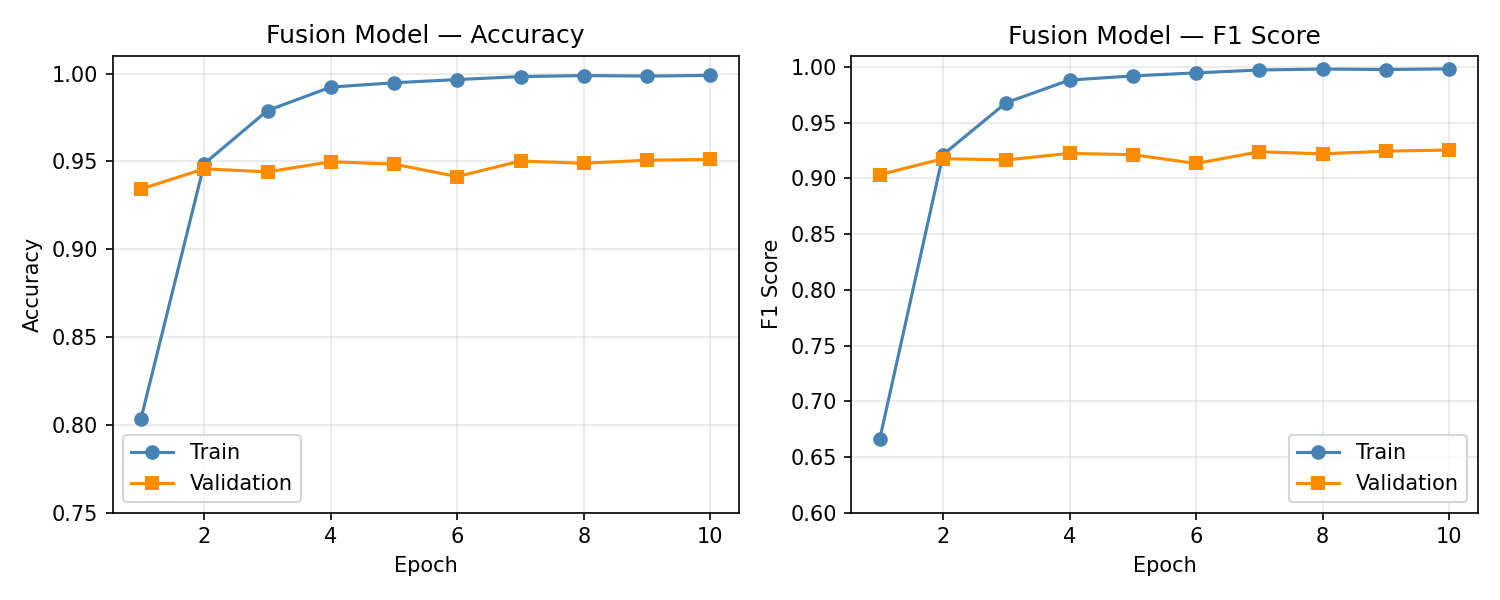
\includegraphics[width=\columnwidth]{training_curves.png}
\caption{Training and validation accuracy (left) and F1 score (right) for the fusion model over 10 epochs.}
\label{fig:training}
\end{figure}

\subsection{Localization}

The localization head achieves 86.9\% pointing accuracy on the 750 incoherent test images (our target was 45\%). Pointing accuracy is the fraction of samples where the highest-scoring patch falls inside the ground-truth alien bounding box. Without the localization loss, pointing accuracy was only 12.9\% --- the classification loss alone does not teach the model \emph{where} to look.

Figure~\ref{fig:heatmaps} shows example heatmaps. When the model correctly detects an incoherent image, the heatmap tends to be tightly focused on the alien object. On missed detections the heatmap is more diffuse, sometimes highlighting the right area but with low confidence.

\begin{figure}[t]
\centering
\begin{subfigure}{0.48\columnwidth}
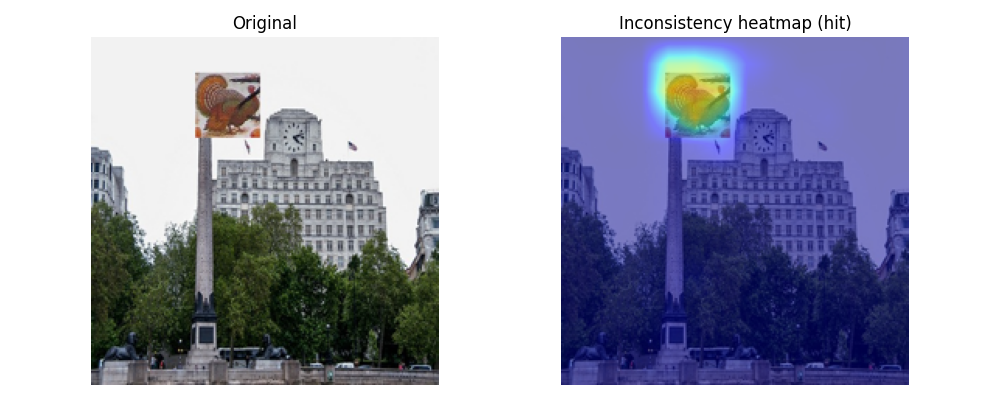
\includegraphics[width=\textwidth]{heatmap_hit_000.png}
\caption{Correct detection}
\end{subfigure}
\hfill
\begin{subfigure}{0.48\columnwidth}
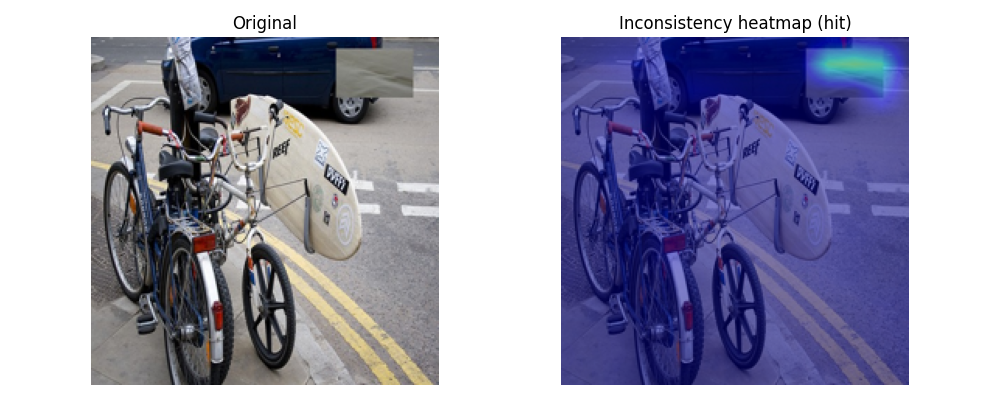
\includegraphics[width=\textwidth]{heatmap_hit_001.png}
\caption{Correct detection}
\end{subfigure}
\\[6pt]
\begin{subfigure}{0.48\columnwidth}
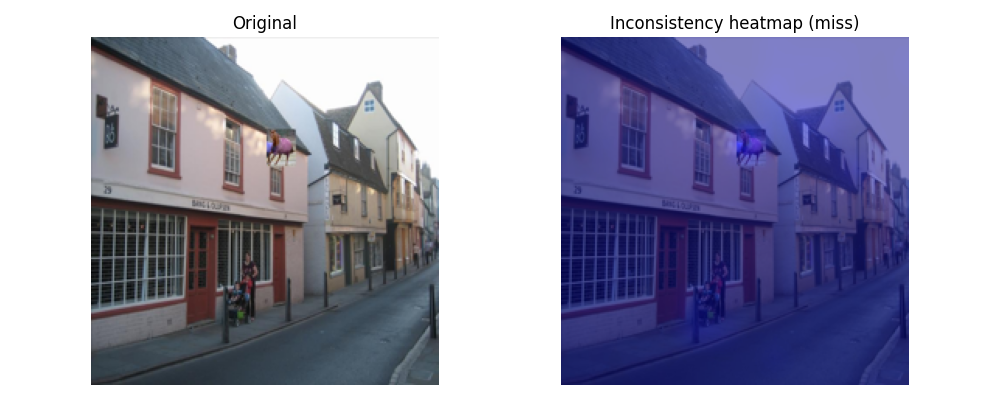
\includegraphics[width=\textwidth]{heatmap_miss_000.png}
\caption{Missed detection}
\end{subfigure}
\hfill
\begin{subfigure}{0.48\columnwidth}
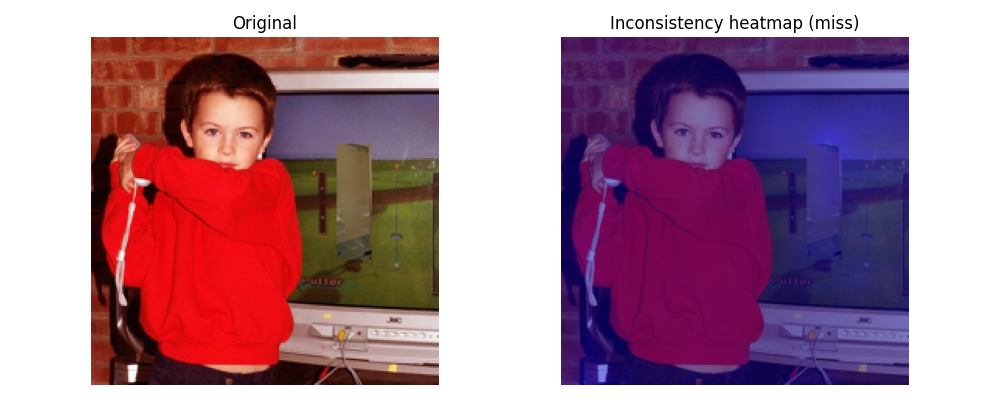
\includegraphics[width=\textwidth]{heatmap_miss_001.png}
\caption{Missed detection}
\end{subfigure}
\caption{Inconsistency heatmaps from the fusion model. Left column in each panel shows the original image; right column shows the heatmap overlay. (a, b) Correct detections with focused activations on the alien object. (c, d) Missed detections where the model highlights the wrong region.}
\label{fig:heatmaps}
\end{figure}

% ============================================================================
\section{Discussion}

The F1 improvement from adding the scene graph is small (+0.1\%), but the ROC-AUC gain (+0.3\%) is more telling --- the fusion model produces better-calibrated probabilities. Still, the GAT-only model's complete failure makes it clear that scene-graph structure on its own is too weak for this task. An alien ``turkey'' node in a scene graph is not inherently suspicious; turkeys can plausibly appear in many contexts. The visual artifacts of copy-paste (lighting mismatches, resolution differences, unnatural object placement) are what the ViT picks up on, and those are far more discriminative than anything in the graph.

The localization results are, in our view, the more interesting outcome. Pointing accuracy of 86.9\% means the model can not only flag an image as incoherent but also show where the problem is. The localization loss was the difference: without it, pointing accuracy was 12.9\%, meaning the patch scores were essentially random. Supervising the per-patch head with ground-truth bounding boxes turned a useless output into a reliable one.

One unexpected result was that regularizing the ViT-only model made it worse (84.1\% F1 vs.\ 91.5\% unregularized). Our augmentation pipeline was probably too aggressive for 10,500 training samples. The fusion model handles the same augmentation fine, possibly because the scene-graph branch acts as a stabilizing signal.

There are clear limitations. Copy-paste augmentation introduces visual artifacts (edge seams, lighting inconsistencies) that a model could learn to detect without understanding scene semantics at all. Real-world inconsistencies --- say, an AI-generated image where a person has six fingers --- would be harder because there are no copy-paste artifacts to latch onto. We also rely on VG ground-truth scene graphs; at inference time on arbitrary images, the model falls back to a dummy single-node graph, which means the GAT branch contributes nothing for images outside the VG dataset.

% ============================================================================
\section{Conclusion}

We built a system that classifies photographs as coherent or incoherent and localizes where the inconsistency is. The fusion model reaches 94.4\% accuracy and 91.6\% F1, with 86.9\% pointing accuracy for localization. The ablation study confirms that visual features do most of the work, but the scene-graph branch helps with calibration and training stability.

The most obvious next step is to replace VG ground-truth graphs with predicted scene graphs from a model like RelTR, so the system works on arbitrary images without falling back to a dummy graph. It would also be worth testing on more realistic inconsistencies --- AI-generated images with semantic errors rather than copy-paste composites --- to see how much of the model's performance comes from detecting visual artifacts versus genuine scene understanding.

% ============================================================================
\section*{Acknowledgments}

This project was developed for MSML640 (Computer Vision) at the University of Maryland, Spring 2026. We thank the course instructors for their guidance throughout the project. We used Visual Genome~\cite{krishna2017visual} for data, HuggingFace Transformers~\cite{wolf2020transformers} for the ViT backbone, and PyTorch Geometric~\cite{fey2019fast} for the GAT implementation.

% ============================================================================
\bibliographystyle{IEEEtran}
\begin{thebibliography}{10}

\bibitem{dosovitskiy2020image}
A.~Dosovitskiy, L.~Beyer, A.~Kolesnikov, D.~Weissenborn, X.~Zhai, T.~Unterthiner, M.~Dehghani, M.~Minderer, G.~Heigold, S.~Gelly, J.~Uszkoreit, and N.~Houlsby,
``An image is worth 16x16 words: Transformers for image recognition at scale,''
in \emph{Proc. ICLR}, 2021.

\bibitem{velickovic2018graph}
P.~Veli\v{c}kovi\'{c}, G.~Cucurull, A.~Casanova, A.~Romero, P.~Li\`{o}, and Y.~Bengio,
``Graph attention networks,''
in \emph{Proc. ICLR}, 2018.

\bibitem{krishna2017visual}
R.~Krishna, Y.~Zhu, O.~Groth, J.~Johnson, K.~Hao, J.~Kravitz, S.~Chen, Y.~Kalantidis, L.-J.~Li, D.~A.~Shamma, M.~S.~Bernstein, and L.~Fei-Fei,
``Visual Genome: Connecting language and vision using crowdsourced dense image annotations,''
\emph{Int. J. Comput. Vision}, vol.~123, no.~1, pp.~32--73, 2017.

\bibitem{johnson2015image}
J.~Johnson, R.~Krishna, M.~Stark, L.-J.~Li, D.~A.~Shamma, M.~S.~Bernstein, and L.~Fei-Fei,
``Image retrieval using scene graphs,''
in \emph{Proc. CVPR}, 2015.

\bibitem{xu2017scene}
D.~Xu, Y.~Zhu, C.~B.~Choy, and L.~Fei-Fei,
``Scene graph generation by iterative message passing,''
in \emph{Proc. CVPR}, 2017.

\bibitem{wolf2020transformers}
T.~Wolf, L.~Debut, V.~Sanh, J.~Chaumond, C.~Delangue, A.~Moi, P.~Cistac, T.~Rault, R.~Louf, M.~Funtowicz, J.~Davison, S.~Shleifer, P.~von~Platen, C.~Ma, Y.~Jernite, J.~Plu, C.~Xu, T.~Le~Scao, S.~Gugger, M.~Drame, Q.~Lhoest, and A.~M.~Rush,
``Transformers: State-of-the-art natural language processing,''
in \emph{Proc. EMNLP: System Demonstrations}, 2020.

\bibitem{fey2019fast}
M.~Fey and J.~E.~Lenssen,
``Fast graph representation learning with PyTorch Geometric,''
in \emph{ICLR Workshop on Representation Learning on Graphs and Manifolds}, 2019.

\bibitem{buslaev2020albumentations}
A.~Buslaev, V.~I.~Iglovikov, E.~Khvedchenya, A.~Parinov, M.~Druzhinin, and A.~A.~Kalinin,
``Albumentations: Fast and flexible image augmentations,''
\emph{Information}, vol.~11, no.~2, 2020.

\end{thebibliography}

\end{document}
